\documentclass[11pt,a4paper]{article}
\usepackage{graphicx}
\usepackage{tcolorbox}
\usepackage{xcolor}
\usepackage{geometry}
\usepackage{tikz}
\geometry{margin=0.8in}

% Define colors
\definecolor{mlblue}{RGB}{31, 119, 180}
\definecolor{mlorange}{RGB}{255, 127, 14}
\definecolor{mlgreen}{RGB}{44, 160, 44}
\definecolor{mlred}{RGB}{214, 39, 40}
\definecolor{mlpurple}{RGB}{148, 103, 189}

\title{\Large\textbf{Discovery 1: Pattern Hunters}\\
\vspace{0.3em}
\normalsize Find the Hidden Groups}
\date{}

\begin{document}
\maketitle
\vspace{-2em}

\section*{Look at This}

\begin{center}
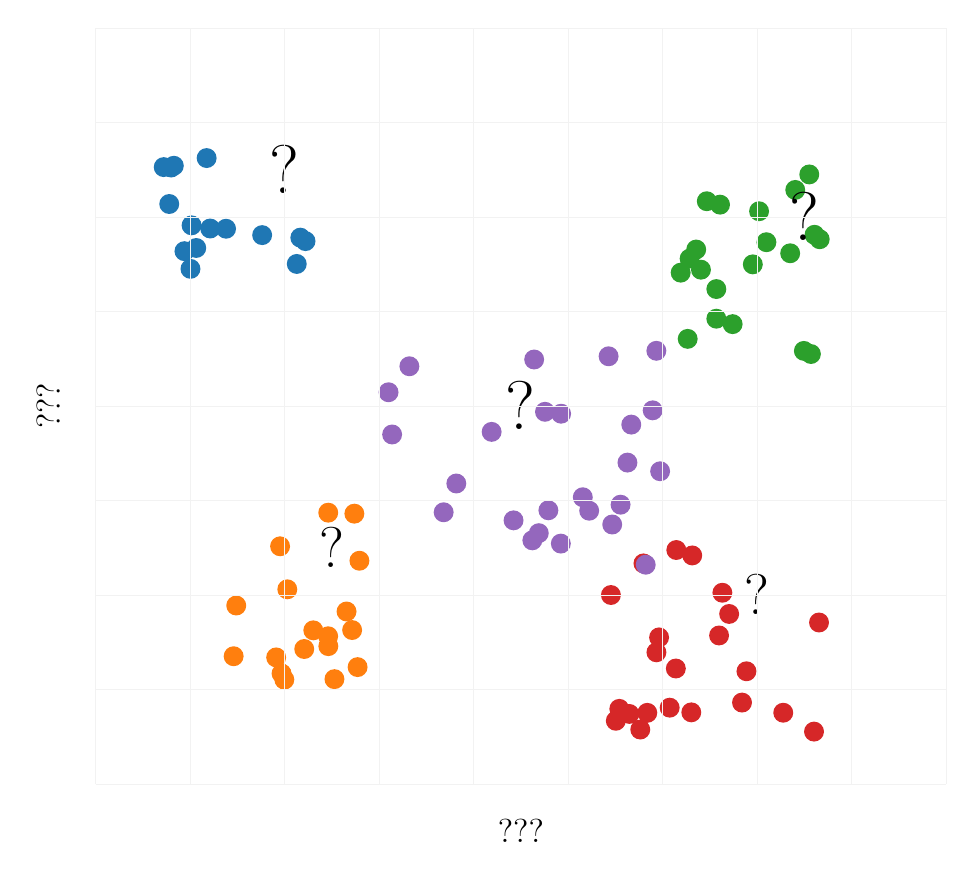
\begin{tikzpicture}[scale=1.2]
% Draw 100 dots representing different items
% Group 1 - Top left cluster (blue items)
\foreach \i in {1,...,15} {
    \pgfmathsetmacro{\x}{1.5 + rand*0.8}
    \pgfmathsetmacro{\y}{6 + rand*0.8}
    \fill[mlblue] (\x,\y) circle (3pt);
}

% Group 2 - Top right cluster (green items)
\foreach \i in {1,...,20} {
    \pgfmathsetmacro{\x}{7 + rand*1}
    \pgfmathsetmacro{\y}{5.5 + rand*1}
    \fill[mlgreen] (\x,\y) circle (3pt);
}

% Group 3 - Bottom left cluster (orange items)
\foreach \i in {1,...,18} {
    \pgfmathsetmacro{\x}{2 + rand*0.9}
    \pgfmathsetmacro{\y}{2 + rand*0.9}
    \fill[mlorange] (\x,\y) circle (3pt);
}

% Group 4 - Bottom right cluster (red items)
\foreach \i in {1,...,22} {
    \pgfmathsetmacro{\x}{6.5 + rand*1.2}
    \pgfmathsetmacro{\y}{1.5 + rand*1}
    \fill[mlred] (\x,\y) circle (3pt);
}

% Group 5 - Center mixed (purple items)
\foreach \i in {1,...,25} {
    \pgfmathsetmacro{\x}{4.5 + rand*1.5}
    \pgfmathsetmacro{\y}{3.5 + rand*1.2}
    \fill[mlpurple] (\x,\y) circle (3pt);
}

% Draw question marks at strategic points
\node[font=\Huge] at (2,6.5) {?};
\node[font=\Huge] at (7.5,6) {?};
\node[font=\Huge] at (4.5,4) {?};
\node[font=\huge] at (2.5,2.5) {?};
\node[font=\huge] at (7,2) {?};

% Grid lines (very faint)
\draw[gray!10, very thin] (0,0) grid (9,8);

% Axis labels
\node[rotate=90] at (-0.5,4) {\large ???};
\node at (4.5,-0.5) {\large ???};
\end{tikzpicture}
\end{center}

\vspace{1em}

\begin{tcolorbox}[colback=mlblue!10, colframe=mlblue!50]
\centering\Large
\textbf{Draw circles around the groups you see}
\end{tcolorbox}

\vspace{2em}

\section*{Now Think}

\begin{center}
\Large
Why did you group them that way?

\vspace{2em}

What if the colors meant nothing?

\vspace{2em}

What if position was random?

\vspace{2em}

\textbf{How many different ways could you group these dots?}
\end{center}

\newpage

\section*{Real World}

\begin{center}
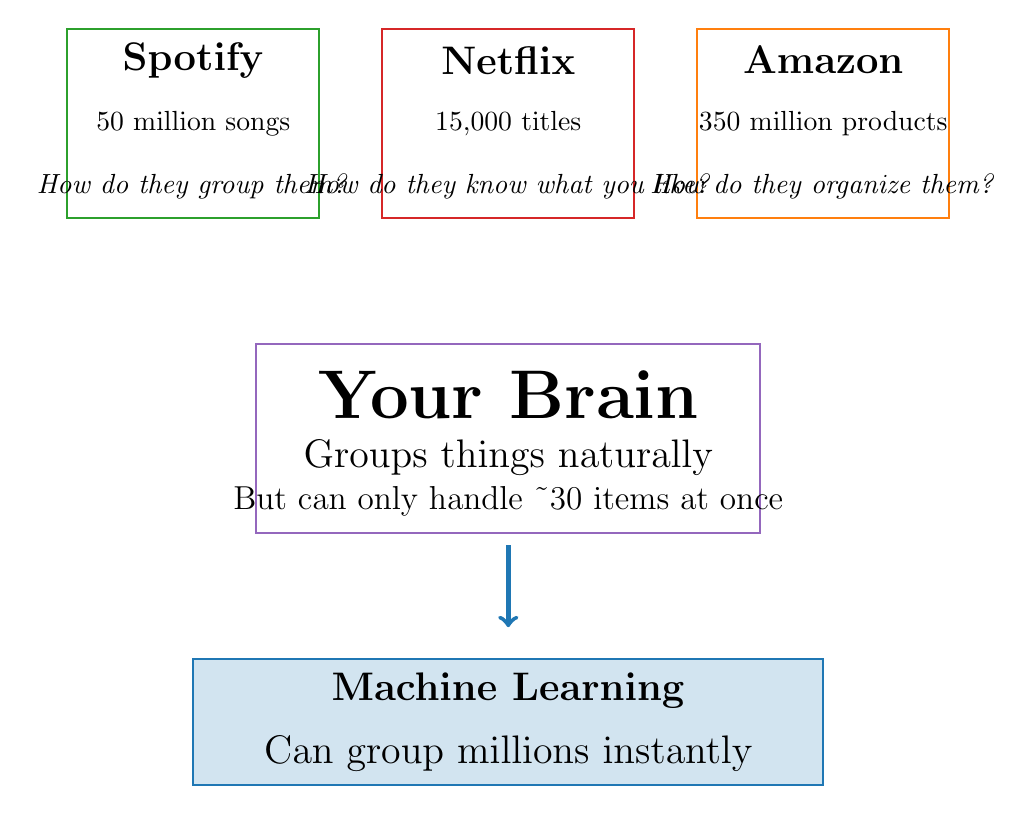
\begin{tikzpicture}[scale=0.8]
% Spotify visualization
\draw[thick, mlgreen] (0,6) rectangle (4,9);
\node at (2,8.5) {\Large\textbf{Spotify}};
\node at (2,7.5) {50 million songs};
\node at (2,6.5) {\textit{How do they group them?}};

% Netflix visualization  
\draw[thick, mlred] (5,6) rectangle (9,9);
\node at (7,8.5) {\Large\textbf{Netflix}};
\node at (7,7.5) {15,000 titles};
\node at (7,6.5) {\textit{How do they know what you like?}};

% Amazon visualization
\draw[thick, mlorange] (10,6) rectangle (14,9);
\node at (12,8.5) {\Large\textbf{Amazon}};
\node at (12,7.5) {350 million products};
\node at (12,6.5) {\textit{How do they organize them?}};

% Your brain
\draw[thick, mlpurple] (3,1) rectangle (11,4);
\node at (7,3.2) {\Huge\textbf{Your Brain}};
\node at (7,2.2) {\Large Groups things naturally};
\node at (7,1.5) {\large But can only handle \textasciitilde30 items at once};

% Arrow pointing down
\draw[->, ultra thick, mlblue] (7,0.8) -- (7,-0.5);

% ML solution
\draw[thick, mlblue, fill=mlblue!20] (2,-1) rectangle (12,-3);
\node at (7,-1.5) {\Large\textbf{Machine Learning}};
\node at (7,-2.5) {\Large Can group millions instantly};
\end{tikzpicture}
\end{center}

\vspace{2em}

\section*{Discovery Challenge}

\begin{center}
\Large
Find 3 examples where you naturally group things:

\vspace{1cm}
1. \underline{\hspace{8cm}}

\vspace{1cm}
2. \underline{\hspace{8cm}}

\vspace{1cm}
3. \underline{\hspace{8cm}}

\vspace{2cm}
\textbf{What would break if these groups didn't exist?}
\end{center}

\vspace{3em}

\begin{tcolorbox}[colback=mlpurple!10, colframe=mlpurple!50]
\centering\large
\textbf{Next Class:} Learn how computers find patterns in chaos
\end{tcolorbox}

\end{document}